\documentclass[fleqn,10pt]{wlpeerj}

\usepackage{todonotes}
\usepackage{url}

\graphicspath{{./figs/}}

\title{CENT - Computer Enabled Neuroplasticity Treatment: a modular, extensible platform for neurofeedback with lightweight wearable EEG devices}

\author[1,2]{Benjamin Cowley}
\author[1]{Jari Torniainen}
\author[2]{Teemu Itkonen}
\affil[1]{Brain{\textbullet}Work Research Centre, Finnish Institute of Occupational Health}
\affil[2]{Cognitive Brain Research Unit, Institute of Behavioural Sciences, University of Helsinki}

\keywords{neurofeedback, electroencephalography, ADHD, computer-enabled, Qt}

\begin{abstract}

Biofeedback/neurofeedback is a growing clinical field. Tools for administering feedback treatment tend to be proprietary and fixed/non-extensible. Thus there is a need for a biofeedback platform which is entirely open source, extensible and free. We present the Computer Enabled Neuroplasticity Treatment (CENT) platform to meet this need.

\end{abstract}

\begin{document}

\flushbottom
\maketitle
\thispagestyle{empty}

\newpage





Story/structure is:
\begin{enumerate}
	\item Introduction + motivation
	\begin{itemize}
		\item we needed a NFB platform and didn't find anything suitable (why not?)
		\item we developed CENT platform at the same time as setting up the clinical trial
		\item we aimed for lots of good things: modular, extensible, state of the art technology, effective but simple UI, minimal but extensible feature set
		\item other systems exist but CENT fills a niche because...
	\end{itemize}

	\item Related work
	\begin{itemize}
		\item Other neurofeedback platforms [DONE!]
		\item Abundance of wearable EEG devices [DONE!]
	\end{itemize}

	\item Architecture - describe the tech. Show where to get it and the compatible parts
	\begin{itemize}
		\item CENT-core
		\item OV-signal proc [DONE!]
		\item CENT-extensions
	\end{itemize}

	\item Validation
	\begin{itemize}
		\item Malmi therapy
	\end{itemize}

	\item Discussion
	\begin{itemize}
		\item We saw a need and filled it
		\item Pros and cons
		\item CENT vs. “Meditation toys”
		\item Usage scenario
		\item Future work: Interfacing with bestest systems (like MIDAS)
	\end{itemize}

	\item Conclusion: CENT platform is great, buy 6!
\end{enumerate}

\newpage




\section{Introduction}

% some motivation
Neurofeedback (NFB) is a growing field, with extensive clinical use, a large body of research literature, and applications also in performance enhancement, entertainment, and stress relief. However tools for administering feedback treatment tend to be proprietary and fixed/non-extensible. Thus there is a need for a biofeedback platform which is both robust, and entirely open source, extensible and free. We present the Computer Enabled Neuroplasticity Treatment (CENT) platform to meet this need.




% some background
\subsection{Background}
NFB, also called electroencephalography (EEG) biofeedback, is operant conditioning of specific temporal, spatial and frequency features extracted from scalp-recorded electrical potentials \citep{Lubar1976}.

NFB has been described as “a mechanism that may be used to stimulate and/or regulate cerebral activity, which in turn may influence cognitive processing” \citep{Vernon2003}. The specific model of effect has been described variously as ‘repairing’ a presumed cause of disorder to ‘normalise’ behaviour, or instead as a tool to enhance cognitive states (see \cite{Gevensleben2014} for a thorough discussion). Either model can be applied in a clinical setting, while the latter enhancement model could also be applied in any non-clinical setting.


%NFB personalisation, qEEG databases
Part of its value is that NFB can be personalized to suit the specific clinical presentation, or performance enhancement requirements, provided that there is requisite theoretical and observational data to guide the personalisation. In clinical settings, the personalisation is often done by reference to quantitative or 'qEEG'-guided normative databases. \cite{Hammond2010} discusses this in detail, illustrating the heterogeneity in qEEG patterns associated with symptoms and discussing the requirements and need for qEEG analysis guided by normative databases. \cite{Johnstone2005} provided a review of such databases, along with a review of qEEG profiles, which are “manifestations seen between genome and behaviour” that they term ‘intermediate’ EEG endophenotypes.


%psychology of NFB
Beside the neurophysiological aspects of NFB, the psychology and experience of NFB are considered by many to be equally important. \cite{Calderon2004} have conceptualized biofeedback as a three-step process that consists of 

\begin{itemize}
	\item becoming aware of a physiological response, 
	\item learning to control the response, and 
	\item transferring control of the response to everyday life.
\end{itemize}

The first two steps of the model - becoming aware and learning to control the electrical activity of the brain - constitute NFB learning. The third step refers to transfer of the NFB learning, often measured in the literature by performance on a neurocognitive test of the treated function (e.g. attention) and/or self-reported symptoms.


%NFB protocols
Two of the more widely-used clinical NFB protocols are ‘theta-beta’ (TB) and ‘sensorimotor rhythm’ (SMR), which are those currently supported in the CENT platform. TB and SMR protocols are based on sub-second frequency-band features.

TB protocol assumes a model where theta power is elevated above normal, and therefore uses an inhibition target for theta power and a reinforcement target for beta power. EEG recording is often at a frontal site. The rationale behind TB training has been described in at least two different ways: as the rectification of cortical hypoarousal \citep{Barry2003}, and as the reinforcement of working memory \citep{Vernon2003}.

SMR protocol reinforces beta power, usually low or mid beta, often with an inhibition target for theta. The site is above the sensorimotor strip, often lateral, such that the beta oscillations correspond to the sensorimotor rhythm. The rationale for SMR training has been proposed as either facilitating attention \citep{Vernon2003}, or the improvement of sleep through an increase in beta spindles, with concomitant effects on cognitive function \citep{Arns2014}.

These protocols contrast with another widely-studied protocol, Slow Cortical Potentials (SCP) training, which feeds back the time domain DC component. SCP targets the Contingent Negative Variation (CNV) Event Related Potential, which \cite{Mayer2015} defined as “a slow negative shift over central sites that develops following the presentation of warning stimulus in expectancy of an imperative stimulus that requires a response”. SCP uses two opposed cortical regulation targets to be trained in random consecutive order. The TB and SMR protocols do not include such an explicit set of counter-poised targets to induce self-regulation, relying instead on a single target of reinforcement/inhibition, which is trained repeatedly.

%more depth to problem statement
\paragraph{Challenges}
The field of NFB makes progress, but in technical terms it does so slowly. The protocols introduced by \cite{Lubar1976} and others have remained unchanged for 40 years. As with any technology, progress relies not just on research, but also on adoption and exploration of the potential by developers. Rapid advances have recently been made in EEG-amplifier hardware and signal processing software, yet the software needed to facilitate open and rapid research and development in clinical NFB is lacking (see below). Opening the field calls for software which is robust, and entirely open source, extensible and free.



% NFB SOFTWARE REVIEW, inc subsections: Neurofeedback software, Wearable EEG sensors
\subsection{Neurofeedback software}
Currently a large number of different NFB software packages exist, most of which are still actively used or still in development. The recent boom of wearable biosensors (such as cheap, commercial EEG devices like the Muse and Melon headbands) has also boosted the number of available personal NFB applications. Despite the popularity, very little literature exists reviewing NFB platforms. One report estimates the usefulness of various BCI frameworks for conducting NFB, and lists design considerations for such a system  \cite{huster2014brain}. In this section we attempt to comprehensively cover different types of software packages are available for NFB.

All available NFB solutions share three basic characteristics which are: 1. a method of interfacing with an EEG device, 2. capability to process the acquired EEG data in real-time and 3. the ability to generate feedback for the user. Outside these parameters different software packages can have vastly different properties. For instance hardware devices supported, licensing, and intended usage all vary greatly between different NFB solutions. The NFB software can roughly be divided into two categories: clinical and non-clinical. The clinical category contains software that is solely intended for various NFB therapies (ADHD therapy being the most common). The other software packages are aimed more for personal cognitive neuromodulation and entrainment (such as mediation and stress management). We have compiled a list (table \ref{nfbsoftware}) which, to our knowledge, contains all of the currently available software packages intended for NFB. 

Table \ref{nfbsoftware} lists 33 NFB software, alongside their respective licenses and other information. 
The 'License' column indicates which license was used when the software was published. In some cases a software package was released with the source code but without a specified license, as noted by a question mark. 
The 'Merit' column refers to scientific merit, defined here as the highest ranking publication the corresponding software was used in. The rankings were extracted from the Finnish Publication Forum, which is a nationally-accepted quality assessment forum for publication channels. Rank values for publication venues are 0 (no rank assigned  by the forum), 1 (basic), 2 (leading), and 3 (highest) \footnote{For more information see \url{http://www.julkaisufoorumi.fi/en/publication-forum}}. The merit value indicates whether the software has been used in NFB related research. For instance the BioExplorer software has been used to study the increase local gamma and beta band activity through NFB \cite{keizer2010enhancing} and the EEGer4 to study the effect of music on alpha/theta NFB \cite{gruzelier2014replication}.

The 'Last Update' column indicates the latest known time of publication for either software or documentation updates. This column indicates whether or not a project is still in active development. Twenty of the software packages are still clearly active (updates less than one year old), and seven more have received updates in the last three years, but the remaining six projects have been dormant for between four and twelve years.

Finally, in the last column the use case for each software (clinical vs non-clinical) is listed. The use case was determined on the basis of the developers' own descriptions from the web-page of the software.

\begin{table}[ht]
\centering
\begin{tabular}{lrrrc}
System & License & Merit & Last Update & Clinical use \\       
\hline
BioEra & Prop. & 1 & 2015-06-22 & No \\   
BrainBay & GPL & 1 & 2014-12-03 & No \\   
BrainAthlon & ? & 1 & 2004-01-01 & No \\   
EEGMIR & ? & 0 & 2003-12-30 & No \\   
ElectricGuru & ? & 0 & 2002-01-21 & No \\   
BioExplorer & Prop. & 2 & 2012-09-26 & No \\  
BioGraph Infiniti & Prop. & 1 & 2013-06-05 & Yes \\
BioTrace+ & Prop. & 2 & 2015-07-23 & Yes \\
BrainFeedbackPro & Prop. & 0 & 2015-11-19 & Yes \\
TruScan Neurofeedback & Prop. & 0 & 2015-11-19 & Yes \\
BrainMaster & Prop. & 1 & 2015-10-09 & Yes \\
BrainPaint & Prop. & 2 & 2012-01-01 & Yes \\
Cygnet & Prop. & 1 & 2015-11-01 & Yes \\
eBioo & Prop. & 0 & 2015-03-01 & Yes \\
EEGer4 & Prop. & 2 & 2013-06-10 & Yes \\
EventIDE & Prop. & 0 & 2015-08-18 & No \\
Mind Workstation & Prop. & 0 & 2011-08-31 & Yes \\
MindReflector & Prop. & 0 & 2013-09-19 & Yes \\
Neurofield & Prop. & 1 & 2015-02-06 & Yes \\
neuromore Studio & Prop. & 0 & 2015-11-06 & No \\
NeurOptimal & Prop. & 0 & 2015-07-01 & Yes \\
NeuroRT & Prop. & 0 & 2015-11-04 & Yes \\
OpenViBE & AGPL & 1 & 2015-10-02 & No \\
SmartMind3 & Prop. & 1 & 2015-01-01 & Yes \\
Melon - Brain Training & Prop. & 0 & 2015-02-28 & No \\
Muse App & Prop. & 0 & 2015-12-16 & No \\
Neurosurfer & Prop. & 0 & 2015-02-15 & Yes \\
BrainWaveOSC & ? & 0 & 2014-07-30 & No \\
OpenNFB & GPL & 0 & 2015-11-19 & No \\
WaveTuner & ? & 0 & 2013-10-16 & No \\
AlphaTrainer & ? & 0 & 2014-05-20 & No \\
Mindrun & MIT & 0 & 2015-09-29 & No \\
Resonanz & GPL & 0 & 2015-07-23 & No \\
\end{tabular}
    \caption{Currently available neurofeedback software packages}\label{nfbsoftware}
\end{table}


Table \ref{nfbsummary} summarises data on license (open-source vs. proprietary) and intended use (clinical vs. non-clinical). This illustrates that the majority of available software are commercial with  proprietary licenses. Although there are almost the same number of clinical and non-clinical software, all of clinical use software have a proprietary license. From this review, it is apparent that there is a clear lack of open-source solutions for clinical NFB. The closest option for such a platform would be the proprietary NeuroRT suite by Mensia Technologies, which like the CENT system, is built on top of the open-source OpenViBE platform. However, there is no NFB software for clinical use that is truly open-source from end-to-end, including both the signal processing back-end and the patient management front-end.


\begin{table}[h]
\centering
\begin{tabular}{lcc}
& Non-clinical  & Clinical \\       
Proprietary & 6 & 15 \\
Open-source  & 11 & 0 \\
\end{tabular}
    \caption{Division of use case and license in neurofeedback software packages}\label{nfbsummary}
\end{table}



\subsection{Wearable EEG sensors} % This section could go to discussion maybe?
In recent years there has been a sharp increase in the availability of ambulatory EEG sensors. This is partly due to technological advances, and also to the popularity of the quantified self movement. The quality of these devices varies from purely consumer-grade (also known as lifestyle applications) to more expensive but near laboratory-grade devices. The suitability of each device for NFB therapy must be tested, but the current trend looks promising as the devices are readily available and cheap compared to laboratory EEG. 

The standard software that usually accompanies these devices seems to be more oriented for self quantification and cognitive enhancement. For instance the MUSE band comes with an application that teaches meditation techniques. Devices like the MUSE, however, provide a communication protocol that allows other software to access the raw data of the device. Therefore, it is plausible that these devices can be used as an input to NFB software. The modification necessary would require that NFB software itself could be modified which further increases the need for open source solutions.


%Our Competition / state of the art…
%Random studies
%%http://musaelab.ca/pdfs/C90A.pdf
%%http://europepmc.org/abstract/med/25882342
%%http://www.ncbi.nlm.nih.gov/pmc/articles/PMC4311636/
%%http://www.sciencedirect.com/science/article/pii/S016787601300247X
%
%paid professional products
%% http://bio-medical.com/products/software.html?dir=asc&order=price
%Neuroelectrics Neurosurfer 'VR' environment
%
%
%23 repos (maybe 2 or 3 decent-looking ones)
%%https://github.com/search?p=1&q=neurofeedback&type=Repositories&utf8=%E2%9C%93
%
%helpful wikipedia page - lists 6 open or GPL warez, inc OpenVIBE
%%https://en.wikipedia.org/wiki/Comparison_of_neurofeedback_software
%
%Free software for specific hardware:
%Nova Tech!
%%http://www.novatecheeg.com/downloads.html
%Vilistus
%%http://www.vilistus.com/software.shtml



% some solution
\subsection{CENT platform}

% development: brief history of CENT use, clinical trial (number)...
The CENT platform was developed to facilitate the CENT clinical trial of NFB treatment for adult ADHD, conducted at the University of Helsinki, Finland \footnote{Clinical trial registered with ISRCTN, DOI 10.1186/ISRCTN13915109}. In the context of the CENT trial, the CENT platform was used with 25 patients, during approximately 40 NFB sessions of 1 hour per patient. Two separate models of EEG amplifier were supported during this trial, along with two NFB protocols (TB and SMR), in two different modes (normal and inverse).  Thus in total eight separate conditions of NFB training were supported by the platform. More detail is given in section \ref{cent:trial} below.

% specifics: CENT platform. Advantages
The CENT platform was designed to connect light-weight EEG amplifiers to a simple, easy-to-use interface for running NFB sessions. The platform's workflow is fixed but adaptable, with configurable settings for personalisation of the treatment, including:
\begin{itemize}
	\item capability to modify the spectral values recorded at baseline, thereby increasing or decreasing difficulty of the task
	\item different games with different levels of stimulation and different 'look and feel'
	\item options to review performance
\end{itemize}

With the existing range of features, the platform demonstrates its utility for the task of clinical neurofeedback. Additionally, with an open, robust, modular architecture it is ideal for extension to add new features or explore other application possibilities.

\paragraph{Outline}
In the rest of this paper, we will first describe in section \ref{methods} the CENT platform, including the core architecture, the signal processing framework, and the options for adding software extensions. Then, in section \ref{cent:trial}, we will describe a validating example of how the platform was used. Finally in section \ref{disc} we discuss the implications for the platform, and possible future work and conclusions.



\section{Methods - Architecture}
\label{methods}
% platform technology
\subsection{Platform architecture}

The CENT platform is built on Qt…
\todo[inline]{todo: platform technology}


%Extensions through OV scenarios is covered in Signal processing section.
\subsection{Signal processing}

\subsubsection{Overview of signal processing architecture}
The signal processing back-end of the CENT system was implemented using the open-souce OpenViBE platform \cite{renard2010openvibe}. The OpenViBE platform consists of a visual modelling language (similar to LabView or Simulink) which enables the design of various signal processing protocols, called \textit{scenarios} in the OpenViBE terminology. The scenarios can be drawn by connecting boxes representing various operations to each other in order to produce to a flowchart of how the data is processed. CENT integrates a fully functional version of OpenViBE which means that the original editor can be used to design new protocols or to modify the existing ones.

The signal processing back-end of the CENT system contains multiple OpenViBE scenarios. A list of scenarios required for a typical NFB session can be found in table \ref{scenariolist}. Scenario-files can be found in the \textit{scenarios} subfolder of the CENT installation. Scenarios themselves are constructed using existing modules known as 'Boxes'. Boxes range from very simple (such as squaring each signal value) to more advanced (such as linear discrimant analysis or support vector machine classifications). Information between boxes is passed as streams of data. OpenViBE has multiple different streams but the two most important for the CENT system are 'Signals' and 'Stimulations'. Signals are simply chunks of EEG data that contain a buffer of the raw voltage values and the sampling rate used to acquire them. Stimulations are similar to trigger codes in most EEG applications and can be used to convey meta information like classification results or signal quality. Most of the common EEG signal analysis operations can be completed using some combination of available boxes and streams. It is important to note that due to the open source nature of OpenViBE it is also possible to write new boxes for desired functionality.

\begin{table}[h]
\centering
\begin{tabular}{ll}
	\hline
	cent\_monitoring\_and\_noise.xml & Scenario for online monitoring of the 
	signal and checking the \\
	&  signal quality \\
	\noalign{\smallskip}
	cent\_baseline.xml & Baseline measurement \\
	\noalign{\smallskip}
	cent\_generate\_configuration.xml & A utlity sceneario used to generate configuration files required for \\
	& the actual session \\
	\noalign{\smallskip}
	cent\_game.xml & The main scenario for the therapy session \\
	\hline
\end{tabular}
    \caption{List of OpenViBE scenarios used in CENT}\label{scenariolist}
\end{table}

Parameters for different boxes can either be set manually in the designer or they can be specified in a separate XML configuration file. Functionality of OpenViBE scenarios can be expanded using scripts written in Lua or Python languages. For more detailed explanation of box configuration see \cite{renard2010openvibe}.

Although the box system is very flexible and gives freedom in experiment design, the implementations of even simple routines tend to require many boxes. For example feature extraction of signal powers from few frequency bands can require the use of multiple boxes. Furthermore the implementation of these processes requires a certain level of knowledge regarding signal processing and might not be intuitive to the end user. For this reason the end user will not need to modify the OpenViBE scenarios in order to use the CENT system. Most of the necessary changes to the parameters can be done from within the CENT system and through configuration files.

The overall aim of the signal processing back-end is to classify the neurological state of the patient, based on power modulations in frequency bands of the EEG. Upper and lower band limits are defined by the protocol in use. In practice classification is done by first acquiring a 60 second baseline recording of resting-state EEG. In the subsequent session the current power values are compared to threshold values extracted from the baseline to generate classifications. Positive classifications occur when changes in the EEG power (registered by the signal analysis module and passed back to the CENT system) in relevant bands matches or exceeds (positively or negatively) the baseline thresholds. Positive classifications modify the behaviour of the game, to give contingent feedback to the patient who thus slowly learns to modify their neural patterns.

\subsubsection{Scenarios}
This section briefly describes the operation of each of the scenario files. Each scenario can be divided into functional sub-elements that correspond to a certain step in a typical BCI processing chain. More information on the behaviour of the sub-elements can be found in the Signal processing protocol section, where structure and behaviour of different components are described.

\paragraph{Monitoring and noise}
Monitoring scenario is responsible for displaying the live EEG and current noise level at the beginning of the therapy session. This scenario is mainly a tool for making sure that the electrodes are properly fixed and that the data streaming is working. Figure \ref{monitoringnoise} shows the structure of the scenario. The scenario structure is relatively simple consisting only of acquisition client, filters and a noise calculator. The same structure is integrated into baseline and game scenarios.

\begin{figure}[h]
	\centering
	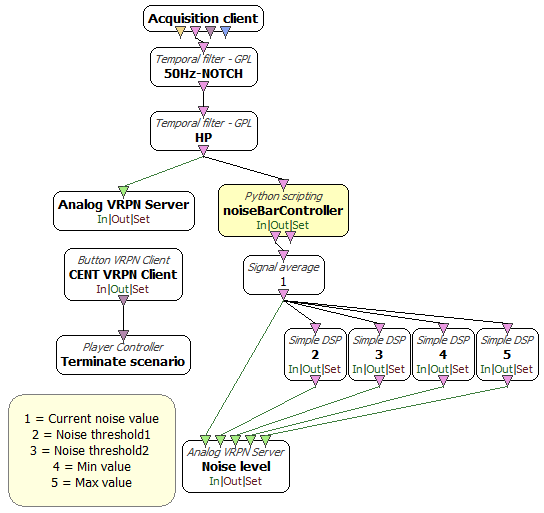
\includegraphics[scale=0.4]{noise.png}
	\caption{OpenViBE scenario for signal and noise check.}\label{monitoringnoise}
\end{figure}  

\paragraph{Baseline}
Baseline scenario is used to determine the baseline frequency-band power values. During the baseline recording patient will be fixating on a cross displayed by the CENT system. Therapist screen will display the live EEG as well as the noise bar. Duration of the baseline recording is 60 seconds with 10 second offsets at the beginning and end of the recording. The recorded data is split to segments of 5 seconds and for each segment the power values are calculated using the same procedure as in the game scenario (this procedure is explained in greater detail in section NN). Finally the segments are are averaged to produce the final baseline values for the session. In addition to the baseline values a complete power spectrum is calculated using the entire recording. Both the baseline values and the spectrum are displayed after the baseline recording for quality assurance.

\begin{figure}[h]
	\centering
	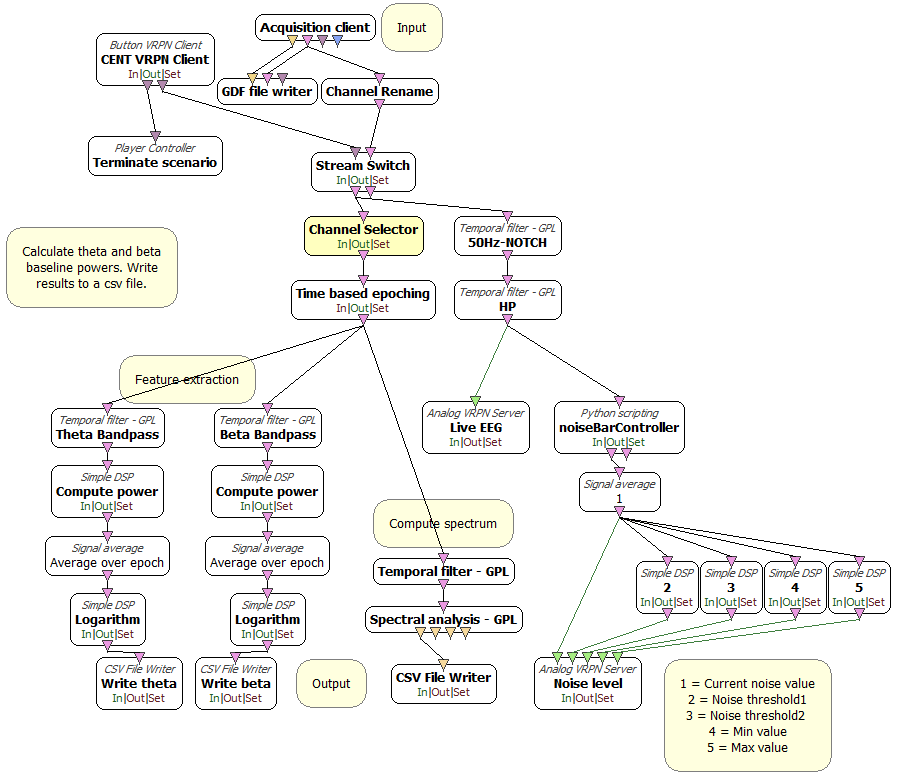
\includegraphics[scale=0.3]{baseline.png}
	\caption{OpenViBE scenario for baseline measurement.}
\end{figure}  

\paragraph{Generate configuration}
Configuration generation scenario is a utility tool used to generate configuration files for the feature extraction in the game trial. The scenario displays no data and the execution only lasts seconds. The scenario takes the baseline values calculated in the previous section and uses them to automatically configure the main game trial. Figure \ref{configuration} displays the corresponding OpenViBE implementation.

\begin{figure}[h]
	\centering
	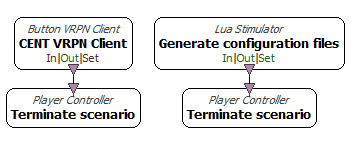
\includegraphics[scale=0.4]{config.png}
	\caption{OpenViBE scenario for writing configuration files.}\label{configuration}
\end{figure}  

\paragraph{Game}
Game scenario evaluates the current mental state of the patient and send information back to CENT. The scenario calculates power values for theta and beta using 1 second epochs and compares them to the values calculated during baseline measurement. The game scenario does not actually do anything related to the game as the actual game mechanics are handled by an external plugin. The OpenViBE implementation of the game trial is visible in figure \ref{processingsections}

  
\subsubsection{Signal Processing Protocol}
NFB signal processing protocol is closely related to the protocol used with brain-computer interfaces (BCI). It thus follows that the signal processing operations performed in a NFB session can be described by borrowing terminology from the field of BCI. In BCI a typical signal processing protocol is divided into four different steps: preprocessing, feature extraction, classification and translation. Preprocessing consists of removing noise and other artifacts from the signal. Feature extraction removes unecessary parts of the signal and classification assigns one of the predefined classes to the incoming signal. Finally the translation performs the action related to the assigned class (such as moving a cursor etc.). In NFB instead of a translation a feedback signal is sent back to the patient i.e, the game reacts to the current neural state. Different signal processing sections of the game scenario have been highlighted in figure \ref{processingsections}. The operation of each section is covered in the following sections.

\begin{figure}[h]
	\centering
	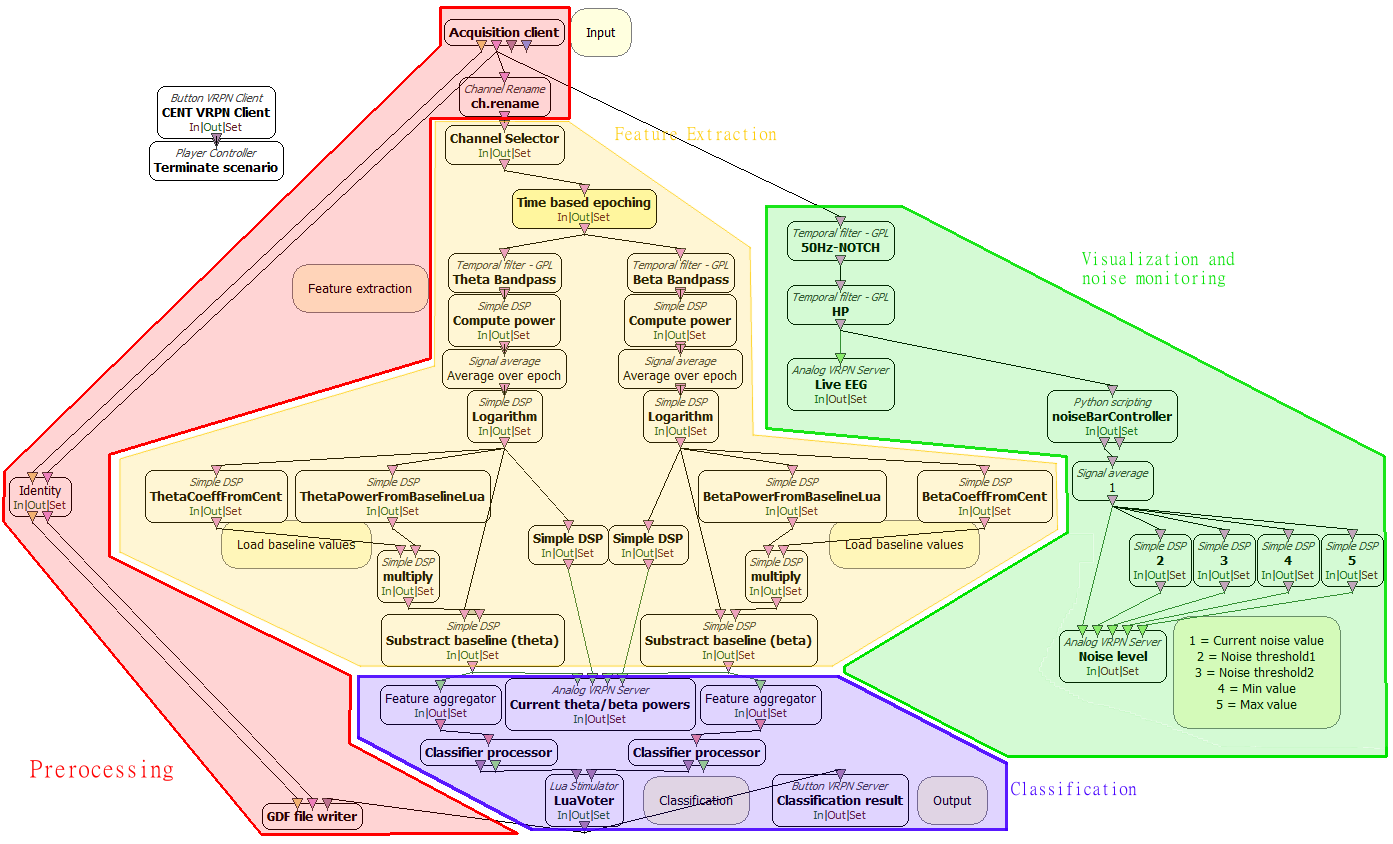
\includegraphics[scale=0.4,angle=90]{sections.png}
	\caption{Signal processing sections of the game scenario.}\label{processingsections}
\end{figure}

\paragraph{Preprocessing}
The EEG signal is passed into OpenViBE through a custom acquistion driver provided by the manufacturer of the EEG device. This driver can send both the EEG data and Stimulation messages to OpenViBE. The EEG device (Enobio) samples the data with internal sampling rate of 250 Hz which is then passed as packages containing several samples to the OpenViBE. The packet size in OpenViBE terminlogy is called a 'chunk' and the size of the chunk can be specified in the software. Multiple chunks can be combined in an epoch of specified length in seconds. Almost all of the OpenViBE scenarios start from the 'Acquisition client'-box which receives data from the acquistion server running under CENT. Acquisition is not a separate scenario but a part of all the signal processing scenarios of the CENT system. Incoming EEG signal is also saved to a GDF file for later analysis. In addition to the data, also the resulting classification labels (stimulations) are registered for each epoch. None of the filters used in visualization or feature extraction are applied to the saved data.

\paragraph{Visualization and noise measurement}
Visualization and noise measurement is used in all of the signal processing scenarios (with the exception of configuration writing). The EEG signal is transmitted from OpenViBE to CENT using a analog VRPN server. Because the EEG signal picks up a lot of noise originating from physiology and the surroundings two filters are applied. First one removes the 50Hz power line interference using a butterworth notch filter (order: 4, stop band: 40-60Hz). Second filter removes the low frequencies physiological artifacts and signal drift. Second filter is a 4th order high pass with a cut-off frequency of 0.5Hz. Noise monitoring is implemented as a separate Python box which provides information to the current signal quality.

\paragraph{Feature extraction}
Feature extraction, in BCI terminology, means extracting the parts of the incoming signal that contain the information relevant to the task. Feature extraction can be thought of as dimensionality reduction where unnecessary components of the signal are removed in order to improve the classifcation accuracy and robustness. In CENT system both the baseline and game scenario have feature extraction structures. In the baseline scenario feature extraction calculates the power of theta and beta bands. Game scenario also computes the two power values but in addition it also compares these values to the baseline values.

Features are extractred from 500ms segments of EEG with 500ms interval. Power values for the two bands in each epoch are extracted using two 4th-order IIR butterworth filters. By default the passbands are the literary values for theta and beta. Alternatively, the two bands can be configured according to the individual alpha frequency of the patient by using configuration files. The use of individual alpha peak frequency is discussed in section NN. Once the incoming signals have been filtered the voltage values are squared and averaged over the epoch. Finally a logarithm is taken to produce the final power values.  

\paragraph{Classification}
Classification assigns the extracted features to one predefined class according to a predefined mathematical rule. In CENT system these classes are ADHD and not-ADHD and the classification is done with 1D Linear Discriminant Analysis (LDA) classifier. Both of the extracted features are classified as either OVTK\_StimulationId\_Target (for not-ADHD) and OVTK\_StimulationId\_NonTarget (for ADHD). Because the version of OpenViBE used in CENT only supports binary classifiers (classifiers with only two possible outputs) the two classifier outputs are combined using a voting classifier implemented in Lua script (luaVoter.lua). 

\subsubsection{System Configuration}
As stated earlier the parameters of the signal processing protocol can be configured using XML formatted configuration files. Configuration files can be found in the IEP directory. The adjustable parameters are listed below along with a description of what they do.

\paragraph{Box configuration}

\begin{description}
\item[noiseBarController] Can set parameters for noise detection. Adjustable parameters are EOG threshold and EOG window. Noise detection is also capable of detecting EMG activity but this feature is not currently used.
\item[Time Based Epoching] Can set the duration of EEG  epochs used in classification. Default value is 500ms with 500ms interval between epochs. Epoch length defines the amount of data used for each classification but also sets the interval of feedback to the patient
\item[Theta/Beta Bandpass] Can adjust the bandpass filters used to calculate powers in theta and beta bands. See IAF section for configuring the passbands according to the individual alpha frequency.
\item[Classifier processor] Can change the classification algorithm and parameters for the two classification processors. The two currently supported algorithms are Linear discriminant analysis and Support vector machines. 
\end{description}

\subsubsection{Individual alpha frequency}
In EEG literature the oscillatory activity of the brain is divided into different frequency ranges denoted by letters from the greek alphabet. The activity in different frequency bands correlates to different mental activities. These values, however, represent a grand average over a large population and might not produce the best possible result in NFB when applied to an individual subject. Earlier research suggests that individual variations in the frequency ranges exist among subjects and there is a method for assigning individual frequency bands for different subjects \cite{klimesch1999eeg}. 

\begin{figure}[ht]
	\centering
	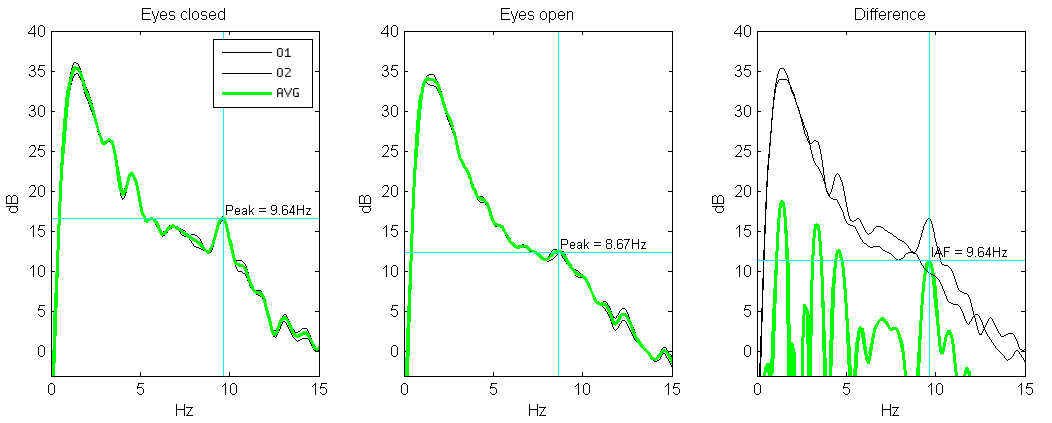
\includegraphics[scale=0.4]{IAF.png}
	\caption{One method for calculating the individual alpha frequency (IAF).}
\end{figure}

In CENT signal analysis individual frequency bands will be determined in the preliminary calibration session of the CENT system to a particular subject. Calibration will consists of recording EEG in eyes-closed condition for few minutes and then analysing the data with an IAF tool also provided in the software package. Alpha peak is extracted from the data by first computing the spectrum and then looking for a peak value in the 7-14 Hz range. Once the peak value has been found other frequency bands can be computed, relative to this peak value (for more details regarding this method see \cite{babiloni2010reactivity}). Once IAF corrected frequency bands have been calculated they can be written into a OpenViBE box configuration files and used in feature extraction. Should the IAF frequency bands not be available or if the calibration fails, frequency bands from the literature are used instead.



% modular, extensible, software additions
\subsection{Software extensions}
\todo[inline]{todo: write about this modular, extensible stuff}




\section{Results - Validation}
\label{cent:trial}

\subsection{Clinical trial}
\lipsum[09]



\section{Discussion}
\label{disc}
\begin{itemize}
	\item We saw a need and filled it
	\item Pros and cons
	\item CENT vs. “Meditation toys”
	\item Usage scenario
	\item Future work: Interfacing with bestest systems (like MIDAS)
\end{itemize}
\lipsum[10] % Dummy text





\subsection{Conclusion}

\lipsum[11] % Dummy text








\section*{Acknowledgments}

Author credits:
\begin{itemize}
	\item BC co-designed the platform UI, designed the clinical trial where it was used, developed the Matlab tool for results review, and co-authored the draft
	
	\item JT co-designed and developed the OpenVibe ‘scenarios’, co-authored the draft, etc, etc [insert what you did]
	
	\item TI tested and debugged the CENT platform, co-authored the draft, etc, etc [insert what you did]
	
\end{itemize}

The authors thank the software engineers:
\begin{itemize}
	\item Arthur Zielazny co-designed the platform UI and the CENT Qt framework

	\item Robert Rabenel co-designed and developed the CENT Qt framework

	\item N. N. co-developed the CENT Qt framework(?) and the movie player application

\end{itemize}

Testers and contributors:
Authors would like to thank Elisa Kallioniemi, Markus Kivikangas, Christina M. Krause, Laura Kauhanen, Mona Moisala and Marko Repo for contributions during design, development and testing.


\newpage

\subsection*{Some \LaTeX{} Examples}
\label{sec:examples}

Use section and subsection commands to organize your document. \LaTeX{} handles all the formatting and numbering automatically. Use ref and label commands for cross-references.

\subsection*{Figures and Tables}

Use the table and tabular commands for basic tables --- see Table~\ref{tab:widgets}, for example. You can upload a figure (JPEG, PNG or PDF) using the project menu. To include it in your document, use the includegraphics command.

\begin{table}[ht]
	\centering
	\begin{tabular}{l|r}
		Item & Quantity \\\hline
		Widgets & 42 \\
		Gadgets & 13
	\end{tabular}
	\caption{\label{tab:widgets}An example table.}
\end{table}


\subsection*{Mathematics}

\LaTeX{} is great at typesetting mathematics. Let $X_1, X_2, \ldots, X_n$ be a sequence of independent and identically distributed random variables with $\text{E}[X_i] = \mu$ and $\text{Var}[X_i] = \sigma^2 < \infty$, and let
$$S_n = \frac{X_1 + X_2 + \cdots + X_n}{n}
= \frac{1}{n}\sum_{i}^{n} X_i$$
denote their mean. Then as $n$ approaches infinity, the random variables $\sqrt{n}(S_n - \mu)$ converge in distribution to a normal $\mathcal{N}(0, \sigma^2)$.

\subsection*{Lists}

You can make lists with automatic numbering \dots

\begin{enumerate}[noitemsep] 
	\item Like this,
	\item and like this.
\end{enumerate}
\dots or bullet points \dots
\begin{itemize}[noitemsep] 
	\item Like this,
	\item and like this.
\end{itemize}
\dots or with words and descriptions \dots
\begin{description}
	\item[Word] Definition
	\item[Concept] Explanation
	\item[Idea] Text
\end{description}

We hope you find write\LaTeX\ useful for your PeerJ submission, and please let us know if you have any feedback. Further examples with dummy text are included in the following pages.


\bibliography{CENTrefs,nfb_software_review,signal_processing}

\end{document}
